% !TEX program = pdflatex
% arara: pdflatex: { shell: false }
% arara: pdflatex: { shell: false }
% arara: latexmk: { options: ["-c"] }
% -------------------------------
\input{inc/_m.latex}
\ShowTOCfalse
% -------------------------------
\nc{\Classe}{2nde}
\nc{\Titre}{Activité : Probabilités}
% -------------------------------

\begin{document}
\Entete

\section{Activité : L'univers des sports}

\begin{wrapfigure}{r}{6cm}\vspace{-7mm}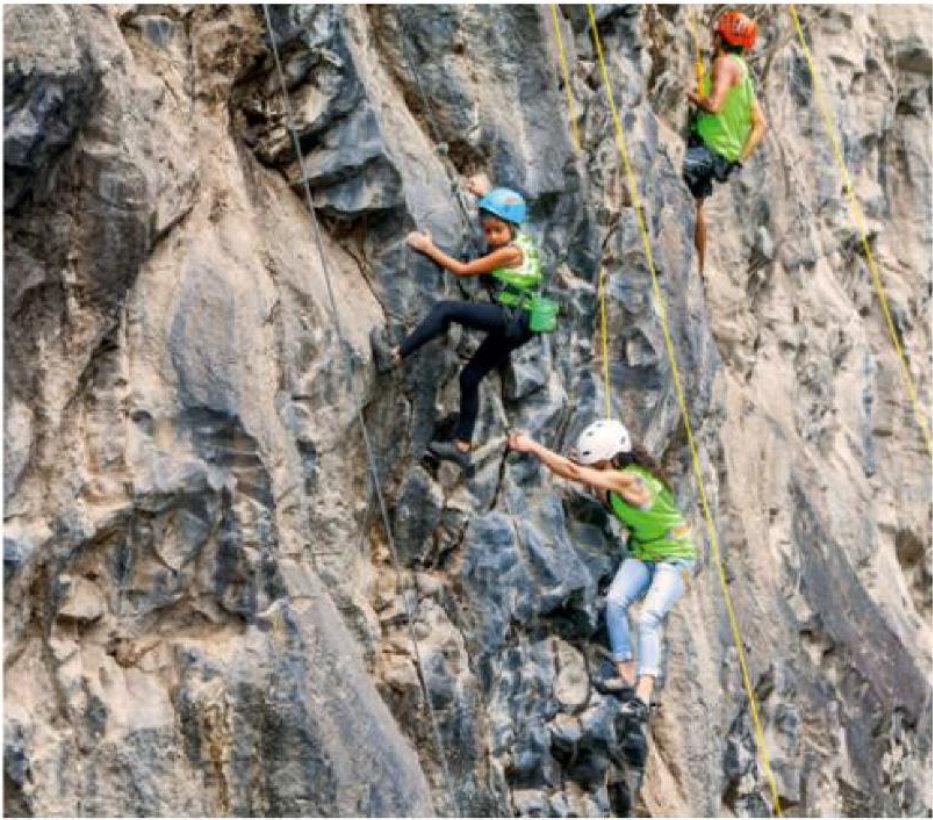
\includegraphics[width=6cm]{img/sport.png}\vspace{-16mm}\end{wrapfigure}
Une colonie de vacances accueille des adolescents âgés de 13 à 17 ans.

Chaque jour, différents sports sont proposés. Ils sont classés en trois catégories :
\bi
\item sports de pleine nature : escalade $(E)$, VTT $(V)$ ;
\item sports individuels : tennis $(T)$, tir à l'arc $(A)$ ;
\item sports collectifs : football $(F)$, handball $(H)$.
\ei

Pour éviter les conflits, les animateurs décident que les adolescents choisiront un sport au hasard.

Arnaud et Véronique sont frère et soeur et ne veulent pas pratiquer le même sport. Ils se demandent la probabilité qu'ils ont d'être dans la même catégorie.
\bigskip
\be
\item \textbf{Premièr jour : tirage sans remise}

Le lundi, les animateurs écrivent la lettre de chaque sport sur différents papiers : ils ont donc six papiers.

Véronique en choisit un au hasard et Arnaud en choisit ensuite un parmi les cinq restants.
\be
\item Justifier qu'il existe $30$ possibilités différentes de répartir Véronique et Arnaud.
\item On estime que la possibilité "Véronique fait du football et Arnaud fait de l'escalade" est identique à "Arnaud fait du football et Véronique fait de l'escalade" car il s'agit de la même paire de sports :$\lbrace F ; E \rbrace$. Parmi les $30$ possibilités, énumérer les $15$ paires de possibilités.
\item Parmi les $15$ paires, quelles sont celles qui indiquent que Véronique et Arnaud vont pratiquer un sport de la même catégorie ?
\item En déduire alors la probabilité qu'ils pratiquent un sport de la même catégorie.
\ee
\ee

\textit{\underline{\faArrowCircleRight\quad Aide :}}
\bi
\item \textit{(a) Déterminer le nombre de choix possibles pour Véronique et, pour chacun de ces choix, déterminer le nombre de choix possibles pour Arnaud.}
\item \textit{(d) Il suffit de calculer la proportion des choix qui nous intéresse sur l'ensemble des choix possibles.}
\ei

\bigskip

\ber
\item \textbf{Deuxième jour : Tirage avec remise}

Le mardi, les animateurs écrivent sur trois papiers les catégories : $1$ ; $2$ ou $3$.

Véronique choisit un papier au hasard et le repose. Arnaud peut donc aussi choisir un papier au hasard parmi les trois.
\be
\item Justifier, à l'aide d'un arbre de dénombrement, qu'il existe 9 possibilités différentes de répartir Véronique et Arnaud.
\ee

Le couple $(1 ; 2)$ signifie que Véronique est dans la catégorie $1$ alors qu'Arnaud est dans la catégorie $2$.

\ber
\item Écrire toutes les possibilités de couples.
\item Parmi tous ces couples, quels sont ceux qui indiquent que Véronique et Arnaud vont pratiquer un sport de la même catégorie ?
\item En déduire alors la probabilité qu'ils pratiquent un sport de la même catégorie.
\ee
\ee

\textit{\underline{\faArrowCircleRight\quad Remarque :}}
\bi
\item \textit{(b) Le couple $(2 ; 1)$ signifie que Véronique est dans la catégorie $2$ alors qu'Arnaud est dans la catégorie $1$.\\Donc les couples $(1 ; 2)$ et $(2 ; 1)$ ne sont pas identiques.}
\ei
\vspace*{5mm}
\begin{center}
	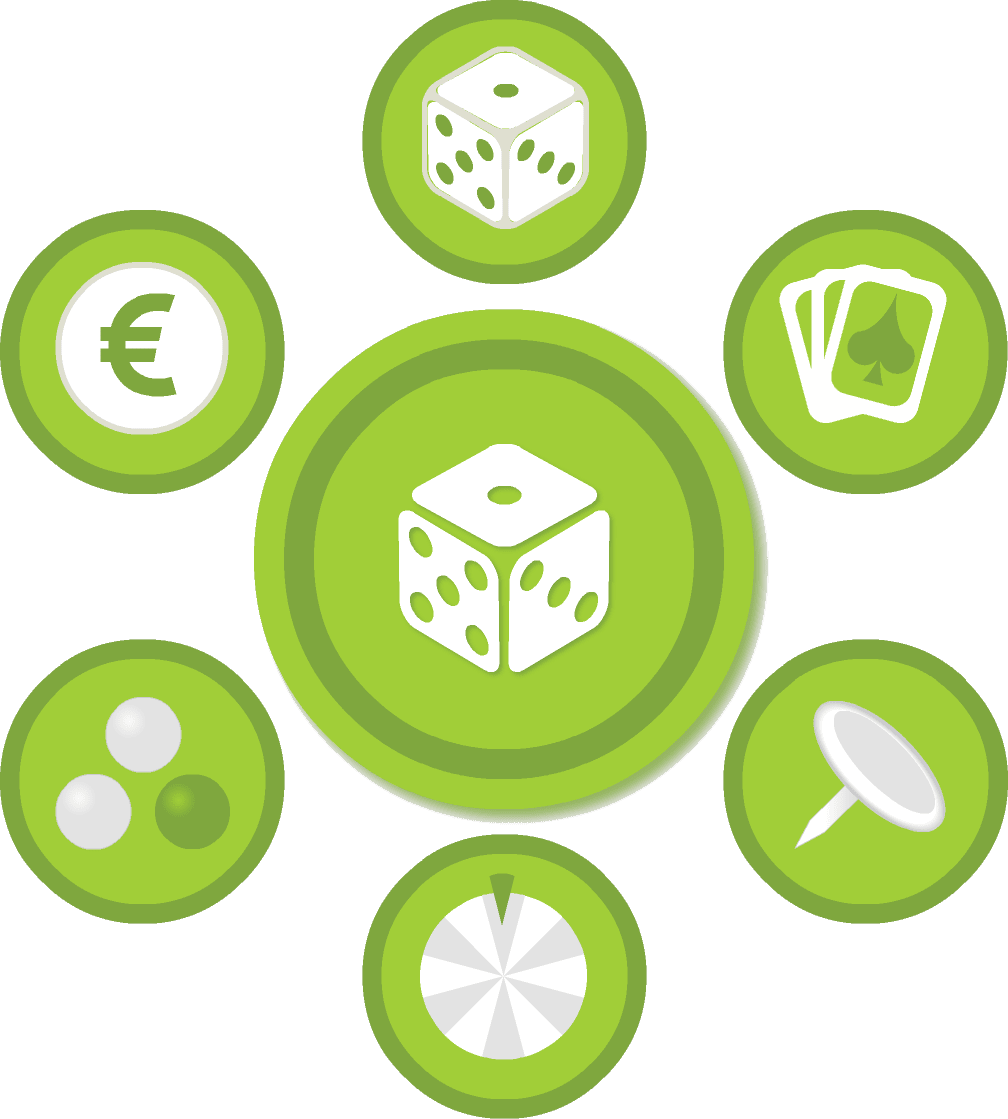
\includegraphics[width=3cm]{img/proba.png}
\end{center}


\end{document}
